\documentclass[a4paper,10pt]{article}
\usepackage{latexsym}
\usepackage[empty]{fullpage}
\usepackage{titlesec}
\usepackage{marvosym}
\usepackage{fontawesome}
\usepackage{hyperref}
\usepackage{enumitem}
\usepackage{xcolor}
\usepackage{amssymb}
\usepackage{graphicx}
\usepackage{tabularx}
\usepackage{array}

\hypersetup{
    colorlinks=true,
    urlcolor=blue
}

\pagestyle{empty}

% Adjust section spacing
\titleformat{\section}{\Large\bfseries}{}{0em}{}[\titlerule]
\titlespacing{\section}{0pt}{2pt}{2pt}

% Set margins
\setlength{\tabcolsep}{0em}
\setlength{\parindent}{0em}
\setlength{\parskip}{0.5em}

% Custom commands
\newcommand{\resumeItem}[1]{\item\small{#1}}
\newcommand{\resumeSubheading}[4]{
  \vspace{1pt}\item
    \textbf{#1} \hfill {#2} \\
    \emph{#3} \hfill {#4} \\
}
\newcommand{\resumeSubItem}[1]{\resumeItem{#1}}
\renewcommand{\labelitemii}{$\circ$}
% Simple checkbox macro (defined early so it can be used in the document)
\newcommand{\checkbox}{\mbox{\framebox[0.4cm][c]{}}}

\begin{document}

%---------- Functional Design Document (CPG Manufacturing Line) ----------
\clearpage
\section*{Changeover Tie Out Tool: Fruit Rollups Line}
\addcontentsline{toc}{section}{Functional Design Document}

\subsection*{Business Context}
Fruit Rollups system is a decoupled manufacturing system (time between 
processing and packaging more than 10 mins) which produces multiple flavor 
SKUs. It has multiple processing and packaging lines. Most of the times 
multiple flavors products are being produced. When producing multiple 
flavor products, flavours are being distributed across line (both 
processing and packaging). Also each line has its own production rate 
since many times lines are getting stopped due to failure of equipments. 
There is a surge belt which accumulates the processed products before 
packaging. When processing rates are higher than packaging rates surge 
belt accunulates and reversely surge accumulation decreases when packaging 
rates are higher than processing rates. Changing over to a new product 
is very challenging as it requires balancing of flavors across lines, 
line rates and surge levels.


\subsection*{Problem Statement}
Fruit Rollups manufacturing system causes overuse or overpack loss during 
changeover to a new product due to below reasons:
\begin{itemize}
  \item Lack of visibility of surge of any flavor
  \item Inefficient distributions of flavors over lines due to human 
  operator's decisions
  \item Unexpected equipment failure causing lines to stop and makes 
  difference in line rates (processing and packaging)
  \item Lack of knowledge on time to stop processing lines.
\end{itemize}
Waste can be minimized by optimizing the flavour distribution, line rate 
and time to stop processing lines.
\\
There is need of a tool at the shop floor to help operators to control
manufacturing operations better and make changeover efficient.

\subsection*{Document metadata}
\begin{tabular}{ l l }
Version: &\ 0.1 \\
Author: & \ Monojit Mandal\\
Date: & \ 2025-12-27\\
\end{tabular}

\subsection*{Executive summary}
A real time mathematical optimization model helps the operator to decide
the optimal time to stop processing lines to reduce overpack or overuse loss.

\subsection*{Scope}
operators are interested to know when to stop processing lines to tackle flavor
imbalance across lines and surge levels. The tool will only provide them the 
recommendations on stoppage time with additional informations like line rates,
surge levels, target production or target time to stop manufacturing.

\subsection*{Stakeholders \& roles}
\begin{tabular}{ l l }
Product Owner: &\ Monojit Mandal \\
Business Stakeholders: & \ Monojit Mandal\\
Technical Stakeholders: & \ Monojit Mandal\\
\end{tabular}

\subsection*{Background \& context}
Operators in Fruit Rollups manufacturing facility reported chanllenges in 
operating the lines due to frequent machine failures of machines and lack of 
visibility in surge level data. Mainly during changeover operators faced 
difficulty to avoid overuse loss. If they could avoid overuse loss they could
ssave 100,000 USD per year

\subsection*{Goals and success criteria}
\begin{itemize}
  \item Overuse Loss: 10--20\% reduction
  \item Monetary Savings: 100,000 USD per year
\end{itemize}

\subsection*{System overview / Architecture}
Fruit Rollups manufacturing system starts with slurry preparation which happens
in drums. There are 4 drums which prepares slurry. Each drum is connected 
to 2 processing lines. Flavours are being added in these processing lines
\begin{figure}[h]
  \centering
  % Include the actual diagram from the assets folder.
  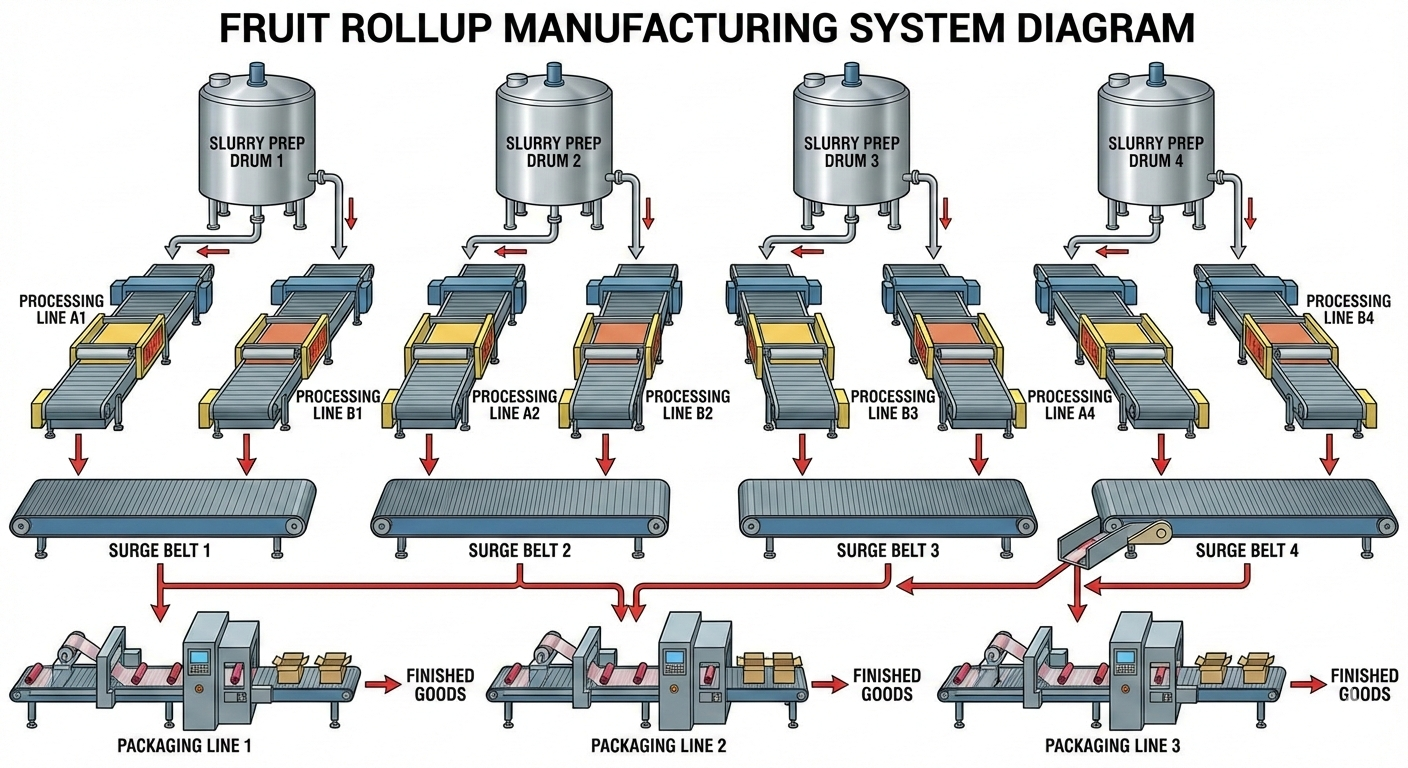
\includegraphics[width=0.9\textwidth]{assets/Gemini_Fruit_Rollups_System.png}
  \caption{System topology (placeholder)}\label{fig:topology}
\end{figure}

\subsection*{Functional components and responsibilities}
For each subsystem include purpose, inputs, outputs, and acceptance criteria. 
Example entries:
\begin{description}
  \item[Conveyors:] Purpose -- product movement and buffering. Inputs -- 
  start/stop, speed setpoint, sensors. Outputs -- encoder feedback, fault 
  signals. Acceptance -- belt speed within $\pm$5\% under load.
  \item[Filling station:] Purpose -- dispense target volume with accuracy. 
  Inputs -- recipe, product ID, level sensors. Outputs -- valve commands, 
  dispense logs. Control -- closed-loop dosing.
  \item[Capping:] Purpose -- apply/torque caps. Include torque checks and 
  presence sensors.
\end{description}

\subsection*{Control strategies and sequences}
Describe PLC state machines and key sequences: start/stop, emergency stop, 
changeover, recipe download and validation, manual/auto modes.

  extbf{Example (sequence):}
\begin{enumerate}
  \item Operator initiates \texttt{LineStart}; PLC verifies interlocks and safety.
  \item PLC starts conveyors and brings machines to ready state.
  \item PLC begins production on first product after recipe verification.
  \item On fault, PLC transitions to \texttt{Fault}; operator resets and returns to \texttt{Idle} or \texttt{Running} depending on checks.
\end{enumerate}

\subsection*{Data model and information flows}
List events and payloads sent to MES/ERP/SCADA. Example fields and a simple table:
\begin{tabularx}{\textwidth}{|l|l|X|}
\hline
Field & Type & Description \\
\hline
productionOrderId & string & MES order identifier \\
productCode & string & SKU / product code \\
timestamp & ISO8601 & event time \\
deviceId & string & PLC or station identifier \\
status & enum & start / stop / fault / complete \\
\hline
\end{tabularx}

Specify data retention policy (e.g., 1s raw data for 90 days, aggregated 
metrics for 3 years).

\subsection*{Interfaces and integration}
Provide an interface table for each integration pair. Template:
\begin{tabularx}{\textwidth}{|>{\raggedright\arraybackslash}p{3.5cm}|>{\raggedright\arraybackslash}p{2.5cm}|>{\raggedright\arraybackslash}X|>{\raggedright\arraybackslash}X|}
\hline
Interface & Protocol & Payload / Format & Direction / Notes \\
\hline
PLC -- SCADA & OPC UA / Modbus & Tag list, alarms, commands & Real-time, cyclic; provide tag mapping appendix \\
SCADA -- MES & REST / MQ & Production events, genealogy & At production events and on changeover \\
MES -- ERP & REST / EDI & Material issue, confirmations & Batch / transactional \\
\hline
\end{tabularx}

\subsection*{PLC \& I/O mapping}
Summarize PLC hardware and provide or link to a detailed I/O matrix (CSV or appendix). Example CSV filename: \texttt{docs/plc\_io.csv}.

\subsection*{Safety and EHS requirements}
List safety devices (light curtains, E-stops, safety PLC), how safety interacts with control logic (safe stop vs immediate stop), interlocks and LOTO procedures, and applicable standards (OSHA, ISO 13849/IEC 61508/62061 as applicable).

\subsection*{Alarms \& HMI requirements}
Define alarm severities, example alarm table, and HMI screens required: Overview, Alarms, Recipes, Maintenance, Diagnostics.

\subsection*{Quality and inspection}
Define inspection points, vision checks, sampling plans and gating rules (e.g., reject a run after X consecutive fails). State what inspection data is logged to MES/historian.

\subsection*{Testing \& validation plan}
  extbf{Unit tests:} function block validation and edge cases.\\newline
  extbf{FAT:} functional sequences, safety tests, integration tests and performance.\\newline
  extbf{SAT:} site verification, environmental checks, full integration with MES/ERP.\\newline
Include acceptance sign-off signature block for stakeholders.

\subsection*{Deployment \& commissioning}
Describe FAT lab requirements, rollout phases, expected downtime, rollback plans and version control practice for PLC/HMI source. Recommend storing PLC/HMI source in a VCS with tags for FAT/SAT/PROD.

\subsection*{Monitoring, telemetry \& maintenance}
KPIs to monitor: OEE, line speed, downtime, MTBF. Define dashboard needs, alerting thresholds, and routine maintenance intervals and spare parts list.

\subsection*{Security}
State network segmentation, firewall rules, user authentication for HMI/SCADA/MES, and secure update procedures for PLC/HMI firmware and application code.

\subsection*{Reliability, availability \& scalability}
Availability targets and redundancy options (redundant PLC, dual network paths). List failure modes and mitigations.

\subsection*{Risk assessment \& mitigations}
Enumerate major risks (single vendor, supply chain, single point of failure) and proposed mitigations.

\subsection*{Open issues / decisions required}
List decisions that need to be made (PLC vendor, MES vendor/integration pattern, mechanical layout sign-off) and owners.

\subsection*{Appendix \& artifacts}
Reference diagrams and files to attach:
\begin{itemize}
  \item Floorplan: \texttt{diagrams/floorplan.png}
  \item Network topology: \texttt{diagrams/network\_topology.png}
  \item PLC rack layout: \texttt{diagrams/plc\_rack.pdf}
  \item I/O matrix: \texttt{docs/plc\_io.csv}
\end{itemize}

\subsection*{Fill-in checklist}
Complete before FAT:
\begin{itemize}
  \item[\checkbox] PLC I/O table attached
  \item[\checkbox] MES interface spec attached
  \item[\checkbox] Safety plan reviewed and signed
  \item[\checkbox] HMI screens mock-ups provided
\end{itemize}

% End of Functional Design Document
\end{document}
\subsection*{Next steps \& recommended deliverables}
\begin{enumerate}
  \item Populate the "System overview" and "PLC \& I/O mapping" with plant-specific data.
  \item Produce the diagrams referenced in the Appendix and attach them to the repository.
  \item Prepare FAT scripts and test cases using the sequences in this document.
  \item Schedule stakeholder review and update version and sign-off fields.
\end{enumerate}

\subsection*{Notes}
This template can be expanded into subsystem-specific FDDs (e.g., Filling Station FDD) for larger projects. If you'd like, I can: (a) populate this with a concrete bottling-line example, (b) generate a CSV PLC I/O template, or (c) create sequence/state diagrams for key workflows.

% End of Functional Design Document